\documentclass[12pt, a4paper]{article}
\usepackage{ctex}

\usepackage{geometry}
\geometry{a4paper,left=3.17cm,right=3.17cm,top=2cm,bottom=2cm}
\usepackage{chemformula} %化学公式宏包
\usepackage[version=4]{mhchem} %化学公式宏包
\usepackage{siunitx} %数字，单位宏包
\sisetup{
	separate-uncertainty = true,
	inter-unit-product = \ensuremath{{}\cdot{}}
} %单位间加小圆点
\usepackage{tikz} %Tikz绘图包
\usetikzlibrary{cd}
\usetikzlibrary{chains}
\usetikzlibrary{arrows}
\usetikzlibrary{arrows.meta} %画箭头
\usetikzlibrary{commutative-diagrams} %交换图
\usetikzlibrary{positioning,automata}
\usepackage[all]{xy}
\usepackage{booktabs} %三线表
\usepackage{multirow} %合并单元格
\usepackage{makecell} %表格内强制换行
\usepackage{array}
\usepackage{booktabs} %控制表格行高
\usepackage{colortbl}  %彩色表格需要加载的宏包
\usepackage{pifont} % 圆圈数字
\usepackage{amsmath}
\usepackage{unicode-math}
\usepackage{fontspec} %字体
\usepackage{listings} % 代码
\newcommand*{\cred}{\textcolor{red}}

\setmainfont{Times New Roman}
\setmathfont{XITS Math}
\setCJKmainfont{SimSun}[AutoFakeBold, AutoFakeSlant] 

\setlength{\parindent}{0pt} %无缩进
\usepackage{setspace}
\usepackage{fancyhdr} %设置页码
\usepackage{lastpage} %获取总页数
\pagestyle{fancy} %fancyhdr宏包新增的页面风格
\renewcommand\headrulewidth{0pt} %取消页眉中的装饰分割线
\fancyhf{}
\cfoot{\footnotesize 第 \thepage\ 页(共 \pageref{LastPage}页)}%当前页 of 总页数


%微分符号
\makeatletter
\newcommand*{\dif}{\mathop{}\!\mathrm{d}}
\makeatother

%直立积分
\DeclareSymbolFont{EulerExtension}{U}{euex}{m}{n}
\DeclareMathSymbol{\euintop}{\mathop} {EulerExtension}{"52}
\DeclareMathSymbol{\euointop}{\mathop} {EulerExtension}{"48}
\let\intop\euintop
\let\ointop\euointop

%Python代码排版设置
\lstset{
    language=Python, % 设置语言
 breaklines=true, % 自动换行
 backgroundcolor=\color[rgb]{0.96,0.96,0.96},% 背景颜色
 keywordstyle=\bfseries\color[RGB]{40,40,255}, % 设置关键字为粗体，颜色为 RoyalBlue
 morekeywords={}, % 设置更多的关键字，用逗号分隔
 basicstyle = \linespread{1} \ttfamily, % 设置行距，字体
 emph={left,right,mid}, % 指定强调词，如果有多个，用逗号隔开
    emphstyle=\bfseries\color{Rhodamine}, % 强调词样式设置
    commentstyle=\color{black!50!white}, % 设置注释样式，斜体，浅灰色
    stringstyle=\color{blue!90!black}, % 设置字符串样式
    columns=flexible,
    numbers=left, % 显示行号在左边
    numbersep=2em, % 设置行号的具体位置
    numberstyle=\footnotesize \color{gray}, % 设置行号格式
    xleftmargin=0em, % 左边距
    xrightmargin=0em, % 右边距
    aboveskip=0.5em, % 上边距
    % framexleftmargin=2em, 行号在框内
    framesep=1em, % 设置边框与代码的距离
    frame=shadowbox,rulesep=3pt,rulesepcolor=\color{red!20!green!20!blue!20},% 阴影边框
    showstringspaces = false, % 不显示字符串中的空格
    }

\renewcommand*{\lstlistingname}{Code} % 重定义Listing标题



\begin{document}
\begin{spacing}{1.625}


\centerline{{\Large \bf{河北农业大学}}}

\centerline{\bf{\Large 20\underline{24}年春（\quad ）/秋（\ \surd \ ）学期}}

\centerline{\Large \bf 参考答案及评分标准（B）卷}

\centerline{\bf 开课学院：\underline{\ \ \quad 理工系 \quad \ \ } \quad 出\ \ 题\ \ 人：\underline{\quad \qquad \qquad 张斌\quad \qquad \qquad}}

\centerline{\bf 课\ \ 程\ \ 号：\underline{\ \ H05981011\quad} \quad 课程名称：\underline{\quad \qquad 化学反应工程 \qquad \quad }}

{{\noindent} \hspace{-2em} \rule[0pt]{16cm}{0.15em}}\\

\vspace{-2em}
{\bf 一、简答题（共50分）}

1. (10分) 

原料与产物只要其中的一种为连续输入或输出而其余则为分批加入或卸出的操作，属于半间歇操作。
\hfill $\cdots \cdots \cdots (5\text{分})$

要求一种反应物的浓度高而另一种反应物的浓度低时，采用半间歇操作是有利的。需要控制反应温度时，除了通过冷却介质移走热量外，还可采用半间歇操作调节加料速度以控制温度。为了提高某些可逆反应的产品收率，可采用半间歇操作，不断移走产物，
与此同时还可提高反应过程速率。
\hfill $\cdots \cdots \cdots (5\text{分})$

{\bf 评分标准：}

第二问不需要完全一致，合理即可。

2. (10分)

\qquad 目标产物P的选择性：

\qquad $S = \frac{r_\mathrm{P}}{r_\mathrm{P} + r_\mathrm{Q}} = \frac{k_1c_\mathrm{A}c_\mathrm{B}^{0.3}}{k_1c_\mathrm{A}c_\mathrm{B}^{0.3} + k_2c_\mathrm{A}^{0.5}c_\mathrm{B}^{1.3}} = \frac{1}{1 + \frac{k_2}{k_1}c_\mathrm{A}^{-0.5}c_\mathrm{B}}$ \hfill $\cdots \cdots \cdots (4\text{分})$

\qquad $c_\mathrm{B}$越大，Q的选择性越大；$c_\mathrm{A}$越大，Q的选择性越小。所以B应该在高浓度下操作，A应该在低浓度下操作。 \hfill $\cdots \cdots \cdots (3\text{分})$

\qquad 可行的反应器型式及加料方式有（任选其一）：

\begin{figure}[htpb]
    \centering
    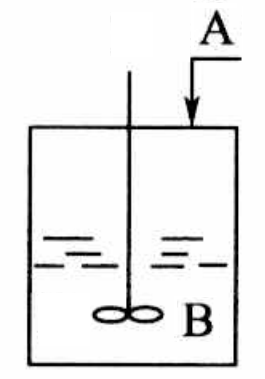
\includegraphics[height=3cm]{images/操作1B} \qquad \qquad 
    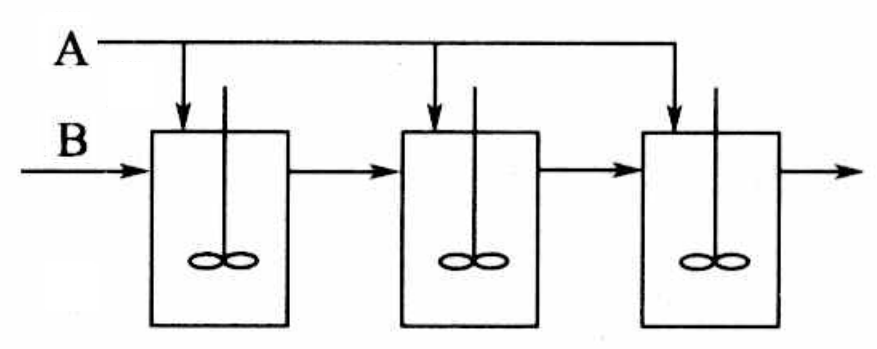
\includegraphics[height=3cm]{images/操作2B}
\end{figure}

\hfill $\cdots \cdots \cdots (3\text{分})$

3. (10分) 

\qquad 绝热温升的意义为：当反应物中的A全部转化时，物系温度升高或降低的度数。\hfill $\cdots \cdots \cdots (4\text{分})$

\qquad 间歇釜式反应器的绝热温升： $\lambda = \frac{n_\mathrm{A0}(-\Delta H_\mathrm{r})}{m_\mathrm{t}\bar{C}_\mathrm{pt}}$  \hfill $\cdots \cdots \cdots (2\text{分})$

\qquad 连续釜式反应器的绝热温升： $\lambda = \frac{c_\mathrm{A0}(-\Delta H_\mathrm{r})}{\rho \bar{C}_\mathrm{pt}}$  \hfill $\cdots \cdots \cdots (2\text{分})$

\qquad 管式反应器的绝热温升： $\lambda = \frac{\omega_\mathrm{A0}(-\Delta H_\mathrm{r})_\mathrm{Tr}}{\bar{C}_\mathrm{pt} M_\mathrm{A}}$  \hfill $\cdots \cdots \cdots (2\text{分})$

4. (10分)

内扩散有效因子反映了内扩散阻力对反应过程的影响，其影响因素有：梯尔模数$\phi$，催化剂颗粒直径，反应速率（反应温度和浓度）。  \hfill $\cdots \cdots \cdots (5\text{分})$

降低内扩散影响的方法有：减小催化剂颗粒直径；优化催化剂孔隙结构，如增大催化剂的孔容和孔半径，增加孔隙率；调整反应条件，如适当提高反应温度或反应物浓度。  \hfill $\cdots \cdots \cdots (5\text{分})$

{\bf 评分标准：}

答出两条即可。


5. (10分)

\begin{itemize}
    \item[(1)] 无论$k_2/k_1$为何值，相同转化率下，间歇釜式反应器P的最大收率总是大于连续釜 \hfill $\cdots \cdots \cdots (4\text{分})$
    \item[(2)] $k_2/k_1$值越小，收率差异越大 \hfill $\cdots \cdots \cdots (2\text{分})$
    \item[(3)] 每一曲线都存在极大值 \hfill $\cdots \cdots \cdots (2\text{分})$
    \item[(4)] 收率总是随着$k_2/k_1$的减小而增大 \hfill $\cdots \cdots \cdots (2\text{分})$
\end{itemize}


{\bf 二、计算题（共50分）}

1. (30分) 

(1) 
$Q_0 = \frac{20000}{24\times 0.8 \times 1} = 1041.67 \ \mathrm{L/h}$ \hfill $\cdots \cdots \cdots (5\text{分})$

$t = \frac{1}{k}\ln \frac{1}{1-X_{\mathrm{A}}} = \frac{1}{2.4}\ln \frac{1}{1-0.8} = 0.67 \ \mathrm{h}$ \hfill $\cdots \cdots \cdots (5\text{分})$

$V_{\mathrm{r}}=Q_{0}(t+t_0)=1041.67\times (0.67+0.5)=1219\mathrm{L}$ \hfill $\cdots \cdots \cdots (5\text{分})$

(2)
$V_{\mathrm{r}}=\frac{Q_{0} c_{\mathrm{A} 0} X_{\mathrm{A}}}{kc_{\mathrm{A0}}(1-X_{\mathrm{A}})}=  \frac{1041.67 \times 0.8}{2.4 \times (1-0.8)}=1736\mathrm{L}$ \hfill $\cdots \cdots \cdots (5\text{分})$

(3)
$V_{\mathrm{r}} = Q_0 \tau = 1041.67\times 0.67 = 698 L$ \hfill $\cdots \cdots \cdots (5\text{分})$

(4) 活塞流反应器反应体积最小，因为活塞流反应器是变速操作，开始时反应速率最大，终了时最小，而且活塞流反应器没有辅助时间，所以活塞流反应器反应体积最小。 \hfill $\cdots \cdots \cdots (5\text{分})$

2. (20分) 

$\phi = \frac{d}{6}\sqrt{\frac{k_\mathrm{p}}{D_\mathrm{eA}}} = \frac{0.5}{6}\sqrt{\frac{0.09}{7.04\times 10^{-4}}} = 0.94$ $\hfill \cdots \cdots \cdots (10\text{分})$

$\eta = \frac{1}{\phi}[\frac{1}{\mathrm{tan}h (3\phi)}-\frac{1}{3\phi}] = \frac{1}{0.94}[\frac{1}{\tanh (3\times 0.94)}-\frac{1}{3\times 0.94}] = 0.694$ $\hfill \cdots \cdots \cdots (10\text{分})$

{\bf 评分标准：}

答案允许存在一定误差。

\end{spacing}
\end{document}